% Тип документа
\documentclass[a4paper,12pt]{extarticle}

% Шрифты, кодировки, символьные таблицы, переносы
\usepackage{cmap}
\usepackage[T2A]{fontenc}
\usepackage[utf8x]{inputenc}
\usepackage[russian]{babel}

% Это пакет -- хитрый пакет, он нужен но не нужен
\usepackage[mode=buildnew]{standalone}

\usepackage
	{
		% Дополнения Американского математического общества (AMS)
		amssymb,
		amsfonts,
		amsmath,
		amsthm,
		% misccorr,
		% 
		% Графики и рисунки
		wrapfig,
		graphicx,
		subcaption,
		float,
		tikz,
		tikz-3dplot,
		caption,
		csvsimple,
		color,
		booktabs,
		pgfplots,
		pgfplotstable,
		geometry,
		% 
		% Таблицы, списки
		makecell,
		multirow,
		indentfirst,
		%
		% Интегралы и прочие обозначения
		ulem,
		esint,
		esdiff,
		% 
		% Колонтитулы
		fancyhdr,
	}  


% Обводка текста в TikZ
\usepackage[outline]{contour}

% Увеличенный межстрочный интервал, французские пробелы
\linespread{1.3} 
\frenchspacing 

 
\usetikzlibrary
	{
		decorations.pathreplacing,
		decorations.pathmorphing,
		patterns,
		calc,
		scopes,
		arrows,
		fadings,
		through,
		shapes.misc,
		arrows.meta,
		3d,
		quotes,
		angles,
		babel
	}


\tikzset{
	force/.style=	{
		>=latex,
		draw=blue,
		fill=blue,
				 	}, 
	%				 	
	axis/.style=	{
		densely dashed,
		blue,
		line width=1pt,
		font=\small,
					},
	%
	th/.style=	{
		line width=1pt},
	%
	acceleration/.style={
		>=open triangle 60,
		draw=magenta,
		fill=magenta,
					},
	%
	inforce/.style=	{
		force,
		double equal sign distance=2pt,
					},
	%
	interface/.style={
		pattern = north east lines, 
		draw    = none, 
		pattern color=gray!60,
					},
	cross/.style=	{
		cross out, 
		draw=black, 
		minimum size=2*(#1-\pgflinewidth), 
		inner sep=0pt, outer sep=0pt,
					},
	%
	cargo/.style=	{
		rectangle, 
		fill=black!70, 
		inner sep=2.5mm,
					},
	%
	caption/.style= {
		midway,
		fill=white!20, 
		opacity=0.9
					},
	%
	}

\newenvironment{tikzpict}
    {
	    \begin{figure}[htbp]
		\centering
		\begin{tikzpicture}
    }
    { 
		\end{tikzpicture}
		% \caption{caption}
		% \label{fig:label}
		\end{figure}
    }


\newcommand{\vbLabel}[3]{\draw ($(#1,#2)+(0,5pt)$) -- ($(#1,#2)-(0,5pt)$) node[below]{#3}}
\newcommand{\vaLabel}[3]{\draw ($(#1,#2)+(0,5pt)$) node[above]{#3} -- ($(#1,#2)-(0,5pt)$) }

\newcommand{\hrLabel}[3]{\draw ($(#1,#2)+(5pt,0)$) -- ($(#1,#2)-(5pt,0)$) node[right, xshift=1em]{#3}}
\newcommand{\hlLabel}[3]{\draw ($(#1,#2)+(5pt,0)$) node[left, xshift=-1em]{#3} -- ($(#1,#2)-(5pt,0)$) }



\newcommand\zi{^{\,*}_i}
\newcommand\sumn{\sum_{i=1}^{N}}

\tikzset{
	coordsys/.style={scale=1.8,x={(1.1cm,-0cm)},y={(0.5cm,1cm)}, z={(0cm,0.8cm)}},
	coordsys/.style={scale=1.5,x={(0cm,0cm)},y={(1cm,0cm)}, z={(0cm,1cm)}}, 
	coordsys/.style={scale=1.5,x={(1cm,0cm)},y={(0cm,1cm)}, z={(0cm,0cm)}}, 
}

\usepgfplotslibrary{units}


% Draw line annotation
% Input:
%   #1 Line offset (optional)
%   #2 Line angle
%   #3 Line length
%   #5 Line label
% Example:
%   \lineann[1]{30}{2}{$L_1$}

\newcommand{\lineann}[4][0.5]{%
    \begin{scope}[rotate=#2, blue,inner sep=2pt, ]
        \draw[dashed, blue!40] (0,0) -- +(0,#1)
            node [coordinate, near end] (a) {};
        \draw[dashed, blue!40] (#3,0) -- +(0,#1)
            node [coordinate, near end] (b) {};
        \draw[|<->|] (a) -- node[fill=white, scale=0.8] {#4} (b);
    \end{scope}
}

\newcommand{\lineannn}[4][0.5]{%
    \begin{scope}[rotate=#2, blue,inner sep=2pt, ]
        \draw[dashed, blue!40] (0,0) -- +(0,#1)
            node [coordinate, near end] (a) {};
        \draw[dashed, blue!40] (#3,0) -- +(0,#1)
            node [coordinate, near end] (b) {};
        % \draw[color=white, color=blue] (a) -- node[fill=white, scale=0.8] {#4} (b);
        \draw[->|] (a)++(-0.3,0) -- (a);
        \draw[->|] (b)++(0.3,0) coordinate (xx) -- (b);
        \draw (xx) node[fill=white, scale=0.8, right] {#4};
    \end{scope}
}

% Круговая стрелка относительно центра (дуга из центра)
\tikzset{
  pics/carc/.style args={#1:#2:#3}{
    code={
      \draw[pic actions] (#1:#3) arc(#1:#2:#3);
    }
  },
  dash/.style={
  	dash pattern=on 5mm off 5mm
  }
}

% Среднее <#1>
\newcommand{\mean}[1]{\langle#1\rangle}

\pgfplotsset{
    % most recent feature set of pgfplots
    compat=newest,
}

% const прямым шрифтом
\newcommand\ct[1]{\text{\rmfamily\upshape #1}}
\newcommand*{\const}{\ct{const}}


\usepackage[europeanresistors,americaninductors]{circuitikz}

% Style to select only points from #1 to #2 (inclusive)
\pgfplotsset{select/.style 2 args={
    x filter/.code={
        \ifnum\coordindex<#1\def\pgfmathresult{}\fi
        \ifnum\coordindex>#2\def\pgfmathresult{}\fi
    }
}}


\usepackage{array}
\usepackage{pstool}


%%%%%%%%%%%%%%%%%%%%%%%%%%%%%%%%%%%%%%%%%%%%%%%%%
\makeatletter
\newif\if@gather@prefix 
\preto\place@tag@gather{% 
  \if@gather@prefix\iftagsleft@ 
    \kern-\gdisplaywidth@ 
    \rlap{\gather@prefix}% 
    \kern\gdisplaywidth@ 
  \fi\fi 
} 
\appto\place@tag@gather{% 
  \if@gather@prefix\iftagsleft@\else 
    \kern-\displaywidth 
    \rlap{\gather@prefix}% 
    \kern\displaywidth 
  \fi\fi 
  \global\@gather@prefixfalse 
} 
\preto\place@tag{% 
  \if@gather@prefix\iftagsleft@ 
    \kern-\gdisplaywidth@ 
    \rlap{\gather@prefix}% 
    \kern\displaywidth@ 
  \fi\fi 
} 
\appto\place@tag{% 
  \if@gather@prefix\iftagsleft@\else 
    \kern-\displaywidth 
    \rlap{\gather@prefix}% 
    \kern\displaywidth 
  \fi\fi 
  \global\@gather@prefixfalse 
} 
\newcommand*{\beforetext}[1]{% 
  \ifmeasuring@\else
  \gdef\gather@prefix{#1}% 
  \global\@gather@prefixtrue 
  \fi
} 
\makeatother
%%%%%%%%%%%%%%%%%%%%%%%%%%%%%%%%%%%%%%%%%%%%%%%%%

\geometry		
	{
		left			=	2cm,
		right 			=	2cm,
		top 			=	3cm,
		bottom 			=	3cm,
		bindingoffset	=	0cm
	}

%%%%%%%%%%%%%%%%%%%%%%%%%%%%%%%%%%%%%%%%%%%%%%%%%%%%%%%%%%%%%%%%%%%%%%%%%%%%%%%



	%применим колонтитул к стилю страницы
\pagestyle{fancy} 
	%очистим "шапку" страницы
\fancyhead{} 
	%слева сверху на четных и справа на нечетных
\fancyhead[R]{\labauthors} 
	%справа сверху на четных и слева на нечетных
\fancyhead[L]{Отчёт по лабораторной работе №\labnumber} 
	%очистим "подвал" страницы
\fancyfoot{} 
	% номер страницы в нижнем колинтуле в центре
\fancyfoot[C]{\thepage} 

%%%%%%%%%%%%%%%%%%%%%%%%%%%%%%%%%%%%%%%%%%%%%%%%%%%%%%%%%%%%%%%%%%%%%%%%%%%%%%%

\renewcommand{\contentsname}{Оглавление}

\usepackage{tocloft}
% \renewcommand{\cftpartleader}{\cftdotfill{\cftdotsep}} % for parts
% \renewcommand{\cftsectiondotsep}{\cftdotsep}% Chapters should use dots in ToC
\renewcommand{\cftsecleader}{\cftdotfill{\cftdotsep}}
%\renewcommand{\cftsecleader}{\cftdotfill{\cftdotsep}} % for sections, if you really want! (It is default in report and book class (So you may not need it).
% ---------
% \newcommand{\cftchapaftersnum}{.}%
% \usepackage{titlesec}
% \titlelabel{\thetitle.\quad}
\usepackage{secdot}
\sectiondot{subsection}
\usepackage{setspace}
\usepackage{amsmath}

\DeclareMathOperator{\sinc}{sinc}
\newcommand{\dif}[3]{


\pgfplotstablegetelem{0}{#2}\of#1

% add column LocalDistance
\pgfplotstablecreatecol
    [expr={\thisrow{#2} - \pgfplotsretval}]
    {LocalDistance#3}{#1}

% add column DifferenceDistance
\pgfplotstablecreatecol
    % [expr={-\thisrow{LocalDistance} + \prevrow{LocalDistance}}]
    % [expr={rad(180)}]
    [expr={-\thisrow{LocalDistance#3} + \prevrow{LocalDistance#3}}]
    {#3}{#1}

}
\newcommand{\Exp}[1]{
	\exp\left(#1\right)
}
\newcommand{\Sinc}[1]{
	\sinc\left(#1\right)
}
\newcommand{\Sin}[1]{
	\sin\left(#1\right)
}
\begin{document}

\def\labauthors{Понур К.А., Сарафанов Ф.Г., Сидоров Д.А.}
\def\labgroup{420}
\def\labnumber{320}
\def\labtheme{Дифракций Фраунгофера}
\renewcommand{\vec}{\mathbf}
\renewcommand{\Re}{\operatorname{Re}}
\renewcommand{\Im}{\operatorname{Im}}
\renewcommand{\phi}{\varphi}
\renewcommand{\kappa}{\varkappa}
\renewcommand{\hat}{\widehat}
%%%%%%%%%%%%%%%%%%%%%%%%%%%%%%%%%%%%%%%%%%%%%%%%%%%%%%%%%%%%%%%%%%%%%%%%%%%%%%%
\begin{titlepage}

\begin{center}

{\small\textsc{Нижегородский государственный университет имени Н.\,И. Лобачевского}}
\vskip 1pt \hrule \vskip 3pt
{\small\textsc{Радиофизический факультет}}

\vfill

{\Large Отчет по лабораторной работе №\labnumber\vskip 12pt\bfseries \labtheme}
	
\end{center}

\vfill
	
\begin{flushright}
	{Выполнили студенты \labgroup\ группы\\ \labauthors}%\vskip 12pt Принял:\\ Менсов С.\,Н.}
\end{flushright}
	
\vfill
	
\begin{center}
	Нижний Новгород, \the\year
\end{center}

\end{titlepage}


%%%%%%%%%%%%%%%%%%%%%%%%%%%%%%%%%%%%%%%%%%%%%%%%%%%%%%%%%%%%%%%%%%%%%%%%%%%%%%%
\begin{spacing}{1}
\tableofcontents
\end{spacing}
% \setstretch{1.2}
\newpage
%%%%%%%%%%%%%%%%%%%%%%%%%%%%%%%%%%%%%%%%%%%%%%%%%%%%%%%%%%%%%%%%%%%%%%%%%%%%%%%
 \section{Теоретическая часть}
В данной работе узучается дифракция на следующих объектах: 1) на одной щели, 2) на двух щелях, 3) на решетке ищ нескольких щелей. Наблюдения и измерения производятся при помощи гониометра -- оптического прибора, предназначенного для измерения углов с большой точностью. 

При помощи гониометра изучают угловое распределение интенсивности дифрагированного света. Углы дифракции изменяются оптическим компенсатором (микроскопом с отсчетным микрометром).

При дифракции Фраунгофера на щели интенсивность излучения в плоскости $xy$, перпендикулярной щели, зависит от угла дифракции по закону
\begin{equation}
	I_{\theta}=I_0\frac{\sin^2\frac{kb\sin\theta}{2}}{(\frac{kb\sin\theta}{2})^2},		
\end{equation}
где $I_0$- интенсивность в направлении $\theta=0$, $I_{\theta}$- интенсивность в направлении $\theta$, $b$- ширина щели, $k$- волновое число.

При дифракции Фраунгофера от решетки с периодом $d$ из $N$ одинаковых щелец ширины $b$ зависимость интенсивность $I_{\theta}$ описывается формулой
\begin{equation}
	I_{\theta}=I_0\frac{\sin^2\frac{kb\sin\theta}{2}}{(\frac{kb\sin\theta}{2})^2}
	\cdot
	\frac{\sin^2\frac{Nkd\sin{\theta}}{2}}{\sin^2\frac{kd\sin{\theta}}{2}}	
\end{equation}

Рассмотрим влияние размеров источника света на вид дифракционной картины при дифрауции на двух щелях. В данной работе источником света служит щель коллиматора. Обозначим ширину этой щели $l$, а её угловой размер $\alpha$. %Нужен рис.3!
От каждой точки источника на объект дифракции падает плоская волна и создает в фокальной плоскости дифракционную картину. Крайние точки источника $K$ и $f$ создают картины, центры которых $K'$ и $f'$ смещены относительно друг друга на угловое расстояние $\alpha$. %Рис 3!

Контрастность дифракционных картин характеризуется видимостью
\begin{equation}
	V=\frac{I_{max}-I_{min}}{I_{max}+I_{min}},
\end{equation}
где $I_{max}$- интенсивность в максимуме, $I_{min}$- интенсивность в ближайшем к нему минимуме.

Видимость дифракционной картины от двух щелей зависит от углового размера источника $\alpha$. Если яркость источника одинакова по всей ширине, то при увеличении $\alpha$ первый минимум вилимостти наступит, когда $\alpha$ станет равно $\theta_1$- угловому расстоянию между нелевым и первым максимами. При малых углах
\begin{equation}
	\sin{\theta_1}\simeq\theta_1=\frac{\lambda}{d},\; \alpha=\frac{l}{F}
\end{equation}
здесь $\lambda$- длина световой волны источника, $d$- фокусное расстояние между щелями на экране, $F$- фокусное расстояние линзы коллиматора.

Условие первого минимума имеет вид
\begin{equation}
	\label{eq:3}
	l=\theta_1F=\frac{\lambda F}{d}
\end{equation}
Формула (\ref{eq:3}) даёт возможность определить шишину источника света по найденному опытным путём расстоянию $d$ между щелями, при котором наступает размытие дифракционной картины.

Таким был метод, использованный в 1920 г. Майкельсоном для измерения углового расстояния между компонентами двойной звезды Капеллы и диаметра звезды Бетельгейзе.

\subsection{Вывод уравнения интенсивностей при дифракции Франгофера на решетке}

\begin{figure}[H]
	\centering
	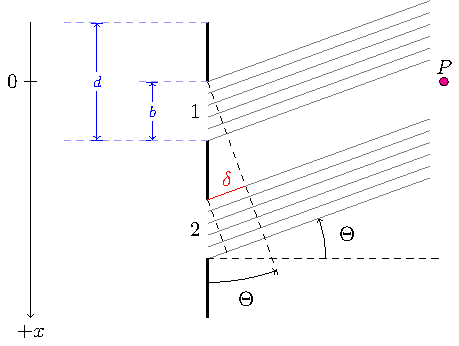
\includegraphics[]{ris/diff}
	\caption{Caption here}
	\label{fig:figure1}
\end{figure}

Сначала выведем дифракцию на первой щели, пользуясь принципом Гюйгенса-Френеля. 

Пусть на щель падает свет амплитудой $E_0$, длиной волны $\lambda$.  Щель разобьем на бесконечно малые излучатели шириной $dx$ и с амплитудой излучаемой волны $\frac{E_0}{b}dx$.  

Набег фазы для каждого такого излучателя относительно излучателя с координатой $x=0$ будет $k\Delta=k\cdot x \sin\Theta$:

\begin{equation}
	d\hat{E}(x)=\frac{\hat{E}_0}{b}\cdot\Exp{i\cdot k x \sin\Theta} dx
\end{equation}
Проинтегрируем по всей щели:
\begin{gather}
	\hat{E}_{1}=\hat{E}_0\int\limits_0^b \frac{1}{i\cdot kb\sin\Theta} \Exp{i\cdot k x \sin\Theta} d[i\cdot k x \sin\Theta]=\\=
	\hat{E}_0 \frac{\Exp{i\cdot k b \sin\Theta}-1}{i\cdot kb\sin\Theta}=
	\hat{E}_0\Exp{i\cdot \frac{k b \sin\Theta}{2}} \frac{\Exp{i\cdot \frac{k b \sin\Theta}{2}}-\Exp{-i\cdot \frac{k b \sin\Theta}{2}}}{i\cdot kb\sin\Theta}=\\=
	\hat{E}_0\Exp{i\cdot \frac{k b \sin\Theta}{2}} \Sinc{\frac{k b \sin\Theta}{2}}
\end{gather}

<<Спрячем>> экспоненту в комплексную амплитуду. Это не повлияет на решение, так как для всех щелей набег фазы в этой экспоненте будет одинаков.

\begin{equation}
	\hat{E}_{1}=\hat{E}_{a}\Sinc{\frac{k b \sin\Theta}{2}}
\end{equation}

Теперь рассмотрим сложение волн, пришедших от всех щелей в дифракционной решетке. Нетрудно показать, что набег фазы будет зависеть от номера щели и угла $\Theta$:
\begin{equation}
	\hat{E}_m=\hat{E}_{1}\Exp{i\cdot k (m-1)d\sin\Theta},
\end{equation}
где $m$ -- номер щели.

Тогда можем записать сумму волн:
\begin{equation}
	\hat{E}(\Theta)=\hat{E}_1 \left(
		1+\Exp{i\cdot kd\sin\Theta}+\ldots+\Exp{i\cdot k (N-1)d\sin\Theta}
	\right)
\end{equation}

Второй множитель здесь -- решеточный множитель, который дает постоянный сдвиг фазы и множитель вида $\sin  Nx / \sin x$. Нетрудно показать, что тогда

\begin{equation}
	\hat{E}(\Theta) \sim \hat{E}_1 \Sinc{\frac{k b \sin\Theta}{2}}
	\left[
		\frac{\Sin{\frac{Nk d \sin\Theta}{2}}}{\Sin{\frac{k d \sin\Theta}{2}}}
	\right]
\end{equation}

И тогда окончательный результат:

\begin{equation}
	\label{eq:intensity}
	I(\Theta) = I_0 \sinc^2\left(\frac{k b \sin\Theta}{2}\right)
	\left[
		\frac{\displaystyle\Sin{\frac{Nk d \sin\Theta}{2}}}{\displaystyle\Sin{\frac{k d \sin\Theta}{2}}}
	\right]^2
\end{equation}

 %%%%%%%%%%%%%%%%%%%%%%%%%%%%%%%%%%%%%%%%%%%%%%%%%%%%%%%%%%%%%%%%%%%%%%%%%%%%%%%
\newpage
\section{Результаты эксперимента}

\subsection{Качественные наблюдения}
\subsubsection{Условия эксперимента}
Изначально свет идет от лампочки накаливания, размер спиральки которой 3 мм.

\subsubsection{Изменение $b$}
С изменением ширины щели решетки -- уменьшением $b$ картинка расширяется, увеличивается расстояние между максимумами

\subsubsection{Изменение $d$}
Экспериментально было установлено, что с изменением периода решетки (уменьшением $d$) картинка расширяется, увеличивается расстояние между максимумами

Теоретически это нетрудно обосновать. Рассмотрим решёточный множитель в формуле (\ref{eq:intensity}). Функция имеет минимумы в точках 
\begin{equation}
  \sin{\theta_m}=\frac{\lambda m}{Nd},\: m=1,2\dots\frac{Nd}{\lambda}.
\end{equation}

Таким образом, при уменьшении d увеличивается расстояние между максимумами.

\subsubsection{Поворот дифракционной решётки}
С увеличением угла, под которым расположена дифракционная решетка картина расширяется


\subsubsection{Изменение $\lambda$}
Для красного ширина центрального максимума шире, чем для зеленого.
Полушириной центрального максимума будем называть угловое расстояние от $\theta=0$ до ближайшего минимума.
Тогда
\begin{equation}
 	\theta_0=\arcsin\frac{\lambda}{Nd}
 \end{equation} 
 То есть приувеличении длины волны картинка расширяется. Что мы и наблюдали в эксперименте.

\subsubsection{Изменение длины щели источника}
Дифракционная картина при изменении длины щели источника не изменяется. 

\subsubsection{Изменение ширины щели источника}

\begin{table}[H]
	    \caption{Показания микрометра щели источника и ширина щели для разных дифракционных картин: З--щель закрыта, Ч--чёткая дифракционная картина, Р--размытая дифракционная картина}
	    \label{tab:chem1}
	    % \pgfkeys{/pgf/number format/.cd,
		% fixed,  1000 sep={\,}}

	\pgfplotstableread{data/dx.tsv}\mytable
	\pgfplotstableset{
	% multicolumn names, % allows to have multicolumn names
	% header=has colnames,
	dec sep align,
	col sep=tab, % the seperator in our .csv file
	fixed zerofill, 
	% precision=4,			
	empty cells with={\textbf{--}},
	every head row/.style={
	before row={\toprule},
	after row={
		\midrule}
		},
	columns/T/.style={
		column name={З, $z$, мм$\cdot10^{-2}$},
		precision=0		
	},	
	columns/CH/.style={
		column name={Ч, $z$, мм$\cdot10^{-2}$},
		precision=0		
	},	
	columns/R/.style={
		column name={Р, $z$, мм$\cdot10^{-2}$},
		precision=0		
	},
	columns/R2/.style={
		column name={Р, $\Delta x$, мм$\cdot10^{-2}$},
		precision=0		
	},	
	columns/CH2/.style={
		column name={Ч, $\Delta x$, мм$\cdot10^{-2}$},
		precision=0		
	},		
	every last row/.style={after row=\bottomrule},
	every row/.style={after row=\midrule}, 
	% columns={N, deg,min,sec},	
	columns={T,CH,R,CH2,R2}	
	% dec zerofill
	% fixed,fixed zerofill,
	% precision=3
	% every even column/.style={
	% 	% column type/.add={>{\columncolor[gray]{.8}}}{}
	% },
	% every even row/.style={
	% 	before row={\rowcolor[gray]{0.95}}
	% },	
	}
	\centering
	\pgfplotstabletypeset[]{\mytable}
\end{table}

\subsubsection{Порядок следования цветов}
Распределение цветов при дифракции в белом свете: ЗЖК













\subsection{Дифракционные картины для разных решёток}
\subsubsection{Дифракция на одной щели}
\begin{table}[H]
	    \caption{$b=0.52$ мм, $N=1$, по минимумам}
	    \label{tab:chem1}
	    % \pgfkeys{/pgf/number format/.cd,
		% fixed,  1000 sep={\,}}

	\pgfplotstableread{data/N1.tsv}\mytable
	
\dif{\mytable}{deg}{deg2}
\dif{\mytable}{min}{min2}
\dif{\mytable}{sec}{sec2}

\pgfplotstablecreatecol
    % [expr={-\thisrow{LocalDistance} + \prevrow{LocalDistance}}]
    % [expr={rad(180)}]
    % [expr={rad(\thisrow{deg2}+1/60*\thisrow{min2}+1/3600*\thisrow{sec2})*1000}]
    [expr={3600*\thisrow{deg2}+60*\thisrow{min2}+\thisrow{sec2}}]
    {deltas}{\mytable}


\pgfplotstablecreatecol
    % [expr={-\thisrow{LocalDistance} + \prevrow{LocalDistance}}]
    % [expr={rad(180)}]
    % [expr={rad(\thisrow{deg2}+1/60*\thisrow{min2}+1/3600*\thisrow{sec2})*1000}]
    [expr={3600*(\thisrow{deg}-\deltaG)+60*(\thisrow{min}-\deltaM)+\thisrow{sec}-\deltaS}]
    {sec3}{\mytable}

\pgfplotstablecreatecol
    % [expr={-\thisrow{LocalDistance} + \prevrow{LocalDistance}}]
    % [expr={rad(180)}]
    % [expr={rad(\thisrow{deg2}+1/60*\thisrow{min2}+1/3600*\thisrow{sec2})*1000}]
    [expr={\thisrow{deltas}/8}]
    {ddeltas}{\mytable}
% \pgfplotstabletypeset
%     [columns={N,deg,min,sec,deg2, min2,sec2,deltas}]
%     {\mytable}
\pgfplotstableset{
	% multicolumn names, % allows to have multicolumn names
	% header=has colnames,
	dec sep align,
	col sep=tab, % the seperator in our .csv file
	fixed zerofill, 
	% precision=4,			
	empty cells with={\textbf{--}},
	every head row/.style={
	before row={\toprule},
	after row={
		\midrule}
		},
	columns/N/.style={
		column name={N},
		precision=0		
	},	
	columns/deg/.style={
		column name={$\Theta^\circ$},
		precision=0		
	},	
	columns/min/.style={
		column name={$\Theta'$},
		precision=0		
	},	
	columns/sec/.style={
		column name={$\Theta''$},
		precision=0,
		column type/.add={}{|}
	},	
	columns/sec2/.style={
		column name={$\Delta\Theta''$},
		precision=0,
		column type/.add={}{|},
	},	
	columns/min2/.style={
		column name={$\Delta\Theta'$},
		precision=0		
	},	
	columns/deg2/.style={
		column name={$\Delta\Theta^\circ$},
		precision=0,
	},	
	columns/deltas/.style={
		column name={$\Delta\Theta$, $''$},
		precision=0,
		dec sep align,
		% column type = {r}
	},	
	columns/ddeltas/.style={
		column name={погрешность, $''$},
		precision=0,
		dec sep align,
		% column type = {r}
	},	
	every last row/.style={after row=\bottomrule},
	every row/.style={after row=\midrule}, 
	% columns={N, deg,min,sec},	
	columns={N,deg,min,sec,deg2, min2,sec2,deltas, ddeltas,sec3}	
	% dec zerofill
	% fixed,fixed zerofill,
	% precision=3
	% every even column/.style={
	% 	% column type/.add={>{\columncolor[gray]{.8}}}{}
	% },
	% every even row/.style={
	% 	before row={\rowcolor[gray]{0.95}}
	% },	
	}
	\centering
	\pgfplotstabletypeset[]{\mytable}
\end{table}
\begin{figure}[H]
	\centering
	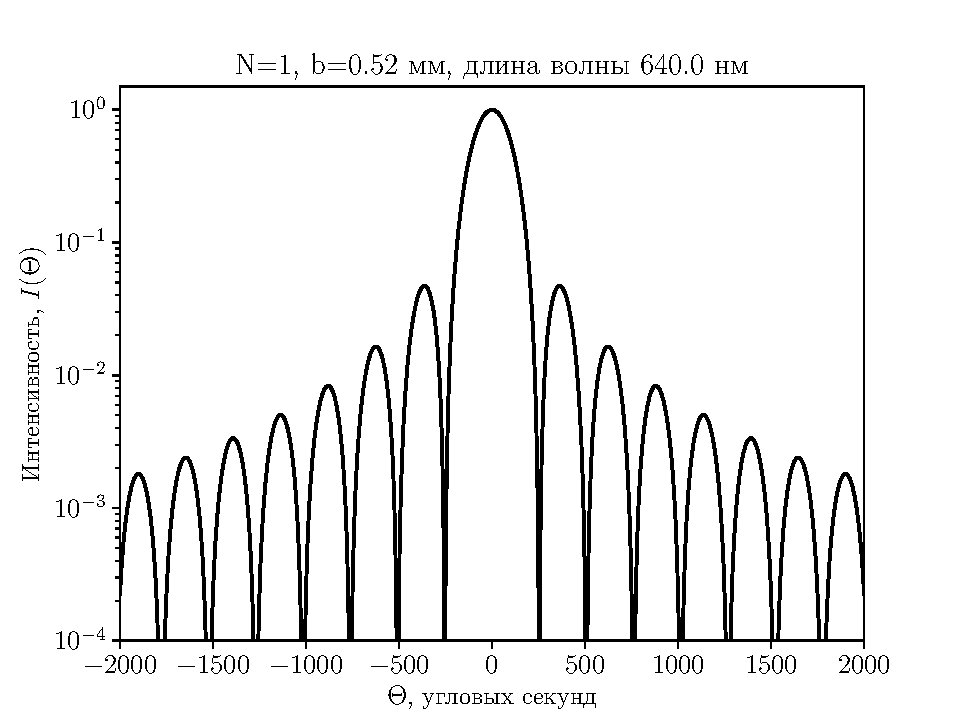
\includegraphics[]{plot/N1}
	\caption{Теоретический вид распределения интенсивности, дифракция на одной щели}
	\label{fig:figure1}
\end{figure}
\subsubsection{Дифракция на двух щелях}

\begin{table}[H]
	    \caption{$b=0.52$ мм, $d=1.5$ мм, $N=2$, по минимумам}
	    \label{tab:chem1} 
	    % \pgfkeys{/pgf/number format/.cd,
		% fixed,  1000 sep={\,}}

	\pgfplotstableread{data/N2.tsv}\mytable
	
\dif{\mytable}{deg}{deg2}
\dif{\mytable}{min}{min2}
\dif{\mytable}{sec}{sec2}

\pgfplotstablecreatecol
    % [expr={-\thisrow{LocalDistance} + \prevrow{LocalDistance}}]
    % [expr={rad(180)}]
    % [expr={rad(\thisrow{deg2}+1/60*\thisrow{min2}+1/3600*\thisrow{sec2})*1000}]
    [expr={3600*\thisrow{deg2}+60*\thisrow{min2}+\thisrow{sec2}}]
    {deltas}{\mytable}


\pgfplotstablecreatecol
    % [expr={-\thisrow{LocalDistance} + \prevrow{LocalDistance}}]
    % [expr={rad(180)}]
    % [expr={rad(\thisrow{deg2}+1/60*\thisrow{min2}+1/3600*\thisrow{sec2})*1000}]
    [expr={3600*(\thisrow{deg}-\deltaG)+60*(\thisrow{min}-\deltaM)+\thisrow{sec}-\deltaS}]
    {sec3}{\mytable}

\pgfplotstablecreatecol
    % [expr={-\thisrow{LocalDistance} + \prevrow{LocalDistance}}]
    % [expr={rad(180)}]
    % [expr={rad(\thisrow{deg2}+1/60*\thisrow{min2}+1/3600*\thisrow{sec2})*1000}]
    [expr={\thisrow{deltas}/8}]
    {ddeltas}{\mytable}
% \pgfplotstabletypeset
%     [columns={N,deg,min,sec,deg2, min2,sec2,deltas}]
%     {\mytable}
\pgfplotstableset{
	% multicolumn names, % allows to have multicolumn names
	% header=has colnames,
	dec sep align,
	col sep=tab, % the seperator in our .csv file
	fixed zerofill, 
	% precision=4,			
	empty cells with={\textbf{--}},
	every head row/.style={
	before row={\toprule},
	after row={
		\midrule}
		},
	columns/N/.style={
		column name={N},
		precision=0		
	},	
	columns/deg/.style={
		column name={$\Theta^\circ$},
		precision=0		
	},	
	columns/min/.style={
		column name={$\Theta'$},
		precision=0		
	},	
	columns/sec/.style={
		column name={$\Theta''$},
		precision=0,
		column type/.add={}{|}
	},	
	columns/sec2/.style={
		column name={$\Delta\Theta''$},
		precision=0,
		column type/.add={}{|},
	},	
	columns/min2/.style={
		column name={$\Delta\Theta'$},
		precision=0		
	},	
	columns/deg2/.style={
		column name={$\Delta\Theta^\circ$},
		precision=0,
	},	
	columns/deltas/.style={
		column name={$\Delta\Theta$, $''$},
		precision=0,
		dec sep align,
		% column type = {r}
	},	
	columns/ddeltas/.style={
		column name={погрешность, $''$},
		precision=0,
		dec sep align,
		% column type = {r}
	},	
	every last row/.style={after row=\bottomrule},
	every row/.style={after row=\midrule}, 
	% columns={N, deg,min,sec},	
	columns={N,deg,min,sec,deg2, min2,sec2,deltas, ddeltas,sec3}	
	% dec zerofill
	% fixed,fixed zerofill,
	% precision=3
	% every even column/.style={
	% 	% column type/.add={>{\columncolor[gray]{.8}}}{}
	% },
	% every even row/.style={
	% 	before row={\rowcolor[gray]{0.95}}
	% },	
	}
	\centering
	\pgfplotstabletypeset[]{\mytable}
\end{table}
\begin{figure}[H]
	\centering
	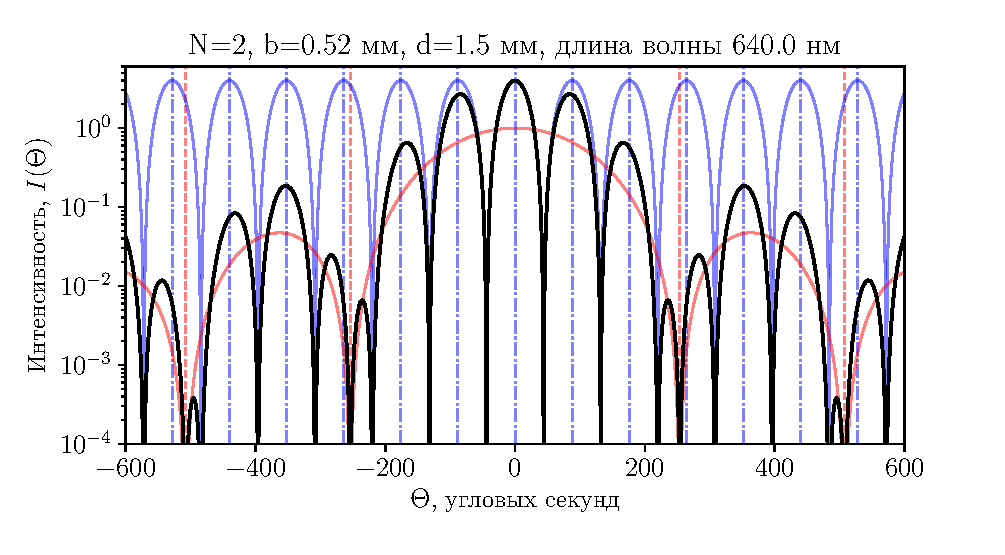
\includegraphics[]{plot/N2}
	\caption{Теоретический вид распределения интенсивности, дифракция на двух щелях}
	\label{fig:figure1}
\end{figure}
\subsubsection{Дифракция на пятнадцати щелях}
\begin{table}[H]
	    \caption{$b=1$ мм, $d=2$ мм, $N=15$, по максимумам}
	    \label{tab:chem1}
	    % \pgfkeys{/pgf/number format/.cd,
		% fixed,  1000 sep={\,}}

	\pgfplotstableread{data/N15.tsv}\mytable
	
\dif{\mytable}{deg}{deg2}
\dif{\mytable}{min}{min2}
\dif{\mytable}{sec}{sec2}

\pgfplotstablecreatecol
    % [expr={-\thisrow{LocalDistance} + \prevrow{LocalDistance}}]
    % [expr={rad(180)}]
    % [expr={rad(\thisrow{deg2}+1/60*\thisrow{min2}+1/3600*\thisrow{sec2})*1000}]
    [expr={3600*\thisrow{deg2}+60*\thisrow{min2}+\thisrow{sec2}}]
    {deltas}{\mytable}


\pgfplotstablecreatecol
    % [expr={-\thisrow{LocalDistance} + \prevrow{LocalDistance}}]
    % [expr={rad(180)}]
    % [expr={rad(\thisrow{deg2}+1/60*\thisrow{min2}+1/3600*\thisrow{sec2})*1000}]
    [expr={3600*(\thisrow{deg}-\deltaG)+60*(\thisrow{min}-\deltaM)+\thisrow{sec}-\deltaS}]
    {sec3}{\mytable}

\pgfplotstablecreatecol
    % [expr={-\thisrow{LocalDistance} + \prevrow{LocalDistance}}]
    % [expr={rad(180)}]
    % [expr={rad(\thisrow{deg2}+1/60*\thisrow{min2}+1/3600*\thisrow{sec2})*1000}]
    [expr={\thisrow{deltas}/8}]
    {ddeltas}{\mytable}
% \pgfplotstabletypeset
%     [columns={N,deg,min,sec,deg2, min2,sec2,deltas}]
%     {\mytable}
\pgfplotstableset{
	% multicolumn names, % allows to have multicolumn names
	% header=has colnames,
	dec sep align,
	col sep=tab, % the seperator in our .csv file
	fixed zerofill, 
	% precision=4,			
	empty cells with={\textbf{--}},
	every head row/.style={
	before row={\toprule},
	after row={
		\midrule}
		},
	columns/N/.style={
		column name={N},
		precision=0		
	},	
	columns/deg/.style={
		column name={$\Theta^\circ$},
		precision=0		
	},	
	columns/min/.style={
		column name={$\Theta'$},
		precision=0		
	},	
	columns/sec/.style={
		column name={$\Theta''$},
		precision=0,
		column type/.add={}{|}
	},	
	columns/sec2/.style={
		column name={$\Delta\Theta''$},
		precision=0,
		column type/.add={}{|},
	},	
	columns/min2/.style={
		column name={$\Delta\Theta'$},
		precision=0		
	},	
	columns/deg2/.style={
		column name={$\Delta\Theta^\circ$},
		precision=0,
	},	
	columns/deltas/.style={
		column name={$\Delta\Theta$, $''$},
		precision=0,
		dec sep align,
		% column type = {r}
	},	
	columns/ddeltas/.style={
		column name={погрешность, $''$},
		precision=0,
		dec sep align,
		% column type = {r}
	},	
	every last row/.style={after row=\bottomrule},
	every row/.style={after row=\midrule}, 
	% columns={N, deg,min,sec},	
	columns={N,deg,min,sec,deg2, min2,sec2,deltas, ddeltas,sec3}	
	% dec zerofill
	% fixed,fixed zerofill,
	% precision=3
	% every even column/.style={
	% 	% column type/.add={>{\columncolor[gray]{.8}}}{}
	% },
	% every even row/.style={
	% 	before row={\rowcolor[gray]{0.95}}
	% },	
	}
	\centering
	\pgfplotstabletypeset[]{\mytable}
\end{table}
\begin{figure}[H]
	\centering
	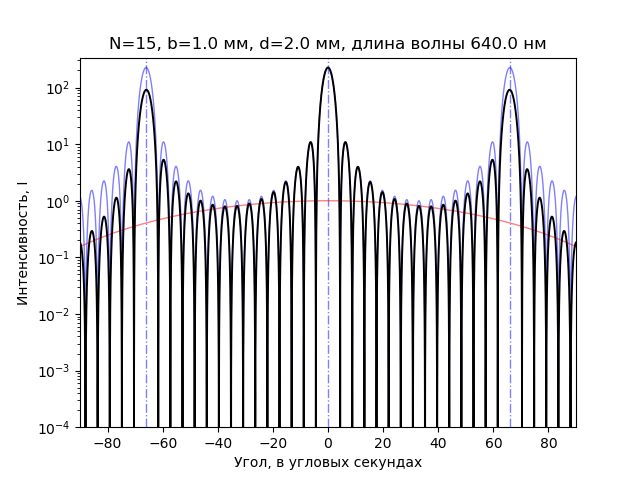
\includegraphics[]{plot/N15}
	\caption{Теоретический вид распределения интенсивности, дифракция на пятнадцати щелях}
	\label{fig:figure1}
\end{figure}



\end{document}